\documentclass[11pt]{article}
\usepackage{graphicx}
\usepackage[utf8]{inputenc} 
\usepackage{epstopdf}
\usepackage[makeroom]{cancel}
\usepackage{framed}
\usepackage{cite}
\usepackage{hyperref}
\usepackage{amsmath}
\usepackage{amsfonts}
\usepackage{bbold}

\begin{document}
\title{FYS4150: Project 3}
\author{Ingrid A V Holm}
\maketitle

\begin{center}
\includegraphics[scale=0.5]{3body_front_cool.png}
\end{center}


\pagebreak

\begin{abstract}
This is an abstract
\end{abstract}






\section{Introduction}

\begin{flushleft}
We wish to solve coupled ordinary differential equations using the Verlet algorithm. From Newton's law of gravitation we get the force between the sun and the earth due to gravitation

\begin{equation}\label{Newton gravitational}
F_G = \frac{G M_{sun} M_{earth}}{r^2} = \frac{M_{earth}v^2}{r}
\end{equation}

where $r$ is the distance between the earth and the sun. We can write this as two separate equations

\begin{equation}
\frac{d^2x}{dt^2} = \frac{F_{G,x}}{M_{earth}}
\end{equation}

\begin{equation}
\frac{d^2y}{dt^2} = \frac{F_{G,y}}{M_{earth}}
\end{equation}

which gives the differential equations

\begin{equation}
\frac{dv_x}{dt} = -\frac{G_{sun}M_{earth}}{r^3} x
\end{equation}

\begin{equation}
\frac{dx}{dt} = v_x
\end{equation}

\begin{equation}
\frac{dv_y}{dt} = - \frac{GM_{sun}}{r^3} y
\end{equation}

\begin{equation}
\frac{dy}{dt} = v_y
\end{equation}

How we define our forces:

\begin{center}
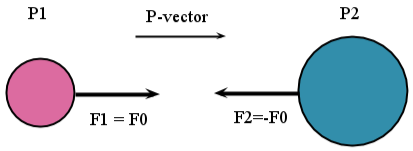
\includegraphics[scale=0.6]{figure1.png}
\end{center}
\end{flushleft}


\section{The Euler method}

\begin{flushleft}
The algorithm for the Euler method is

\begin{equation}
y^{(1)}_{n+1} = y_n^{(1)} + hy_{n+1}^{(2)} + \mathcal{O}(h^2) 
\end{equation}

\begin{equation}
y^{(2)}_{n+1} = y^{(2)}_n +ha_n + \mathcal{O}(h^2)
\end{equation}


where $h = \frac{b-a}{N}$ and $t_{i+1} = t_i + h$. $a_n$ is the acceleration, which also needs to be calculated. For our project this gives: 

\begin{equation}
v_{x,i+1} = v_{x,i} - h \frac{4 \pi^2}{r_i^3} x_i
\end{equation}

\begin{equation}
x_{i+1} = x_i + hv_{x,i}
\end{equation}

\begin{equation}
v_{y,i+1} = v_{y,i} - h \frac{4 \pi^2}{r_i^3} y_i
\end{equation}

\begin{equation}
y_{i+1} = y_i + hv_{y,i}
\end{equation}
\end{flushleft}

\pagebreak

\section{Perihelion precession of Mercury}

\begin{flushleft}
At this point we should ask ourselves - \textit{how well does our model represent the actual planet orbits?} The planets move around the sun in ellipses. Some perturbations of this motion occur due to the gravitational pull of other planets. These cause the orientation of the ellipses to rotate very slowly in space, as illustrated in figure (\ref{Perihelion}). For most planets the observed planet orbits, including these small perturbations, can be explained using Newtonian physics alone. In fact, the only planet for which a significant difference between prediction and observation occurs is Mercury, the smallest, innermost planet of the solar system. The predicted angular velocity of the orientation is off by $43$ arc seconds (angle $\times \frac{1}{3600}$) per century. Albeit a subtle difference, this caused quite a head scratching. We now know the explanation lies in \textit{the theory of general relativity}. Because Mercury lies so close to the Sun, it orbits a region in which spacetime is disturbed by the Sun's mass. We will not go into details (as we do not know them), but introduce an expression for the force between the Sun and Mercury with a relativistic correction

\begin{equation}
F_G  = \frac{G M_{\odot} M_{Mercury}}{r^2} [1 + \frac{3l^2}{r^2c^2}]
\end{equation}

\begin{figure}[ht]
\label{Perihelion}
\begin{center}
\includegraphics[scale=0.4]{fig2.png}
\end{center}
\caption{Mercury's orbit around the sun}
\end{figure}

\end{flushleft}

\section{Changing the center of mass}

\begin{flushleft}
We now have a system consisting of the earth, jupiter and the sun. We want to change the origin to the center of mass, in stead of the position of the sun. We then need to fulfill the conditions

\begin{equation}
\frac{1}{m_1 + m_2 + m_3} (m_1 \vec{r_1} + m_2 \vec{r_2} + m_3 \vec{r_3}) = 0
\end{equation}

\begin{equation}
\vec{p}_1 + \vec{p}_2 + \vec{p}_3 = 0
\end{equation}
\end{flushleft}


\section{Velocity Verlet}

\begin{flushleft}
In the velocity Verlet method the velocity and position are calculated at the same value of the time variable. The basic algorithm is

\begin{equation}
x_{i+1} = x_i + v_i h + \frac{1}{2} a_i h^2
\end{equation}

\begin{equation}
v_{i+1} = v_i + \frac{a_i + a_{i+1}}{2}h
\end{equation}

Apparently, we need some intermediate steps. We therefore divide into 

\begin{equation}
v_{i+1/2} = v_i + \frac{1}{2} a_i h
\end{equation}

\begin{equation}
x_{i+1} = x_i + v_{i+1/2} h
\end{equation}

Calcuate the new acceleration, from $a = F/m$:

\begin{equation}
v_{i+1} = v_i + \frac{1}{2} a_{i+1} h
\end{equation}

\section{Energy and angular momentum conservation}

\begin{flushleft}
A small snippet of program that saves the energies for all time steps in a matrix, and finds the absolute value of the largest error

\begin{equation}
\epsilon_i = \frac{|E_{i, max} - E_{i, min}|}{|E_{i, max}|}
\end{equation}

where $i=0,1,2$ are the total, kinetic and potential energies.
\end{flushleft}

\begin{flushleft}
\textbf{Why should energies and angular momentum be conserved?} For circular motion an $d\vec{r}_{sun}=0$, the speed of the earth $|v_{earth}|$ and the distance between the earth and the sun are constant. Since the potential and kinetic energies are functions of these, they should be constant

\begin{equation}
E_k = \frac{1}{2} m |\vec{v_{earth}}|^2
\end{equation}

\begin{equation}
E_p = \frac{G m_{earth} m_{sun}}{r}
\end{equation}

Angular momentum is also a function of these

\begin{equation}
L = m \vec{r} \times \vec{v}
\end{equation}
\end{flushleft}

\section{Results}

\begin{flushleft}
From including only the earth and the sun for the Euler and Verlet methods:
\begin{center}
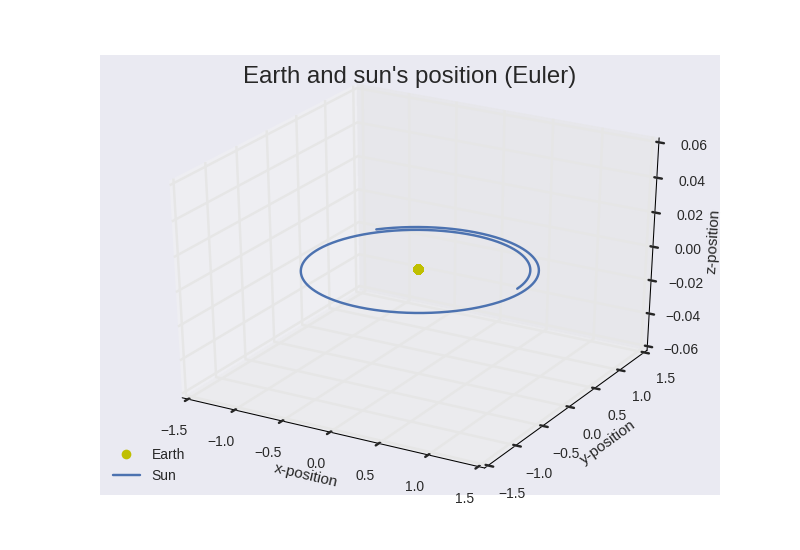
\includegraphics[scale=0.6]{fig1_euler.png}
\end{center}

\begin{center}
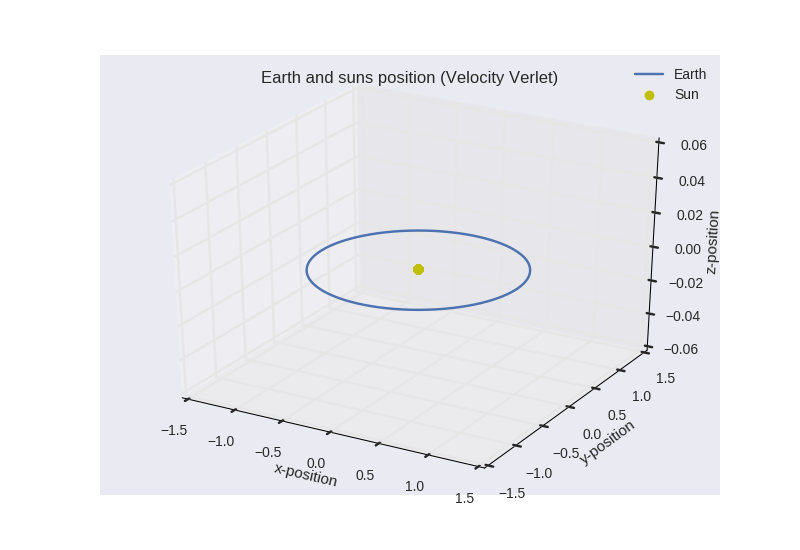
\includegraphics[scale=0.6]{fig1_verlet.png}
\end{center}
\end{flushleft}

\begin{flushleft}
From checking stability of Verlet and Euler by varying the timestep $dt$. For Verlet we see that the movement is circular at $dt= 0.01$, so this overlaps with $dt=0.001$. For Euler, we see that $dt=0.001$ starts to diverge heavily, and $dt=1$ goes almost like a tangent:

\begin{center}
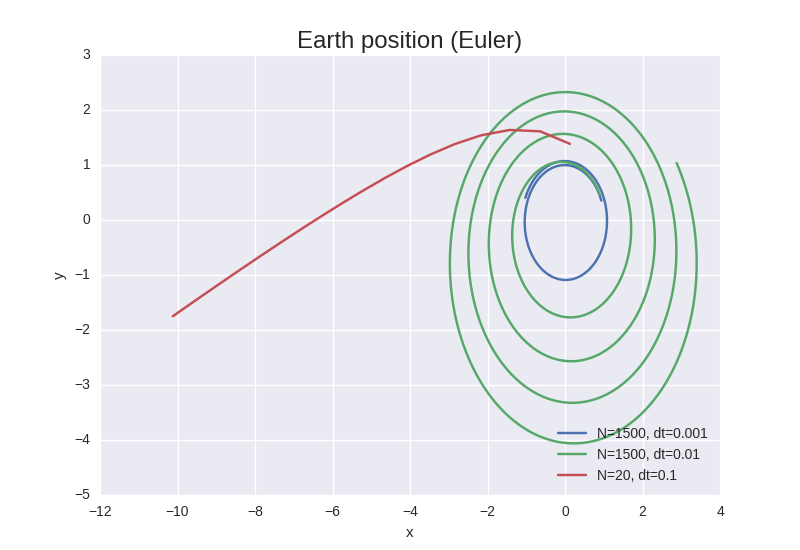
\includegraphics[scale=0.5]{Euler_stability_dt.png}
\end{center}

\begin{center}
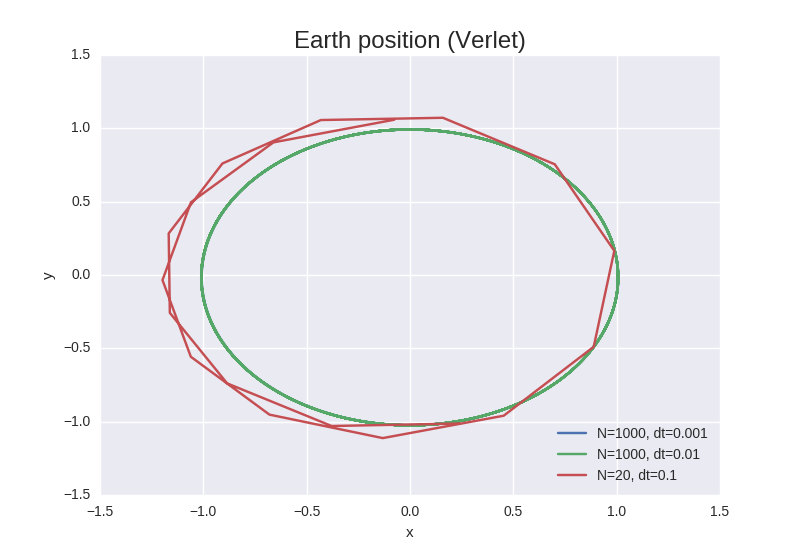
\includegraphics[scale=0.5]{Verlet_stability_dt.png}
\end{center}
\end{flushleft}

\section{3 body (Sun, Earth and Jupiter)}

\begin{flushleft}
The coordinates from NASA already use the center of mass as origin. 

\begin{center}
\includegraphics[scale=0.6]{3body_N14000.png}
\end{center}

Changing the mass of Jupiter:

\begin{figure}
\begin{center}
\includegraphics[scale=0.5]{3body_N14000_m10.png}
\includegraphics[scale=0.5]{3body_N14000_m1000.png}
\end{center}
\end{figure}

We now want to give the sun a velocity so that the total momentum is zero: 

$$
\textbf{v}_{Sun} =- \frac{1}{m_{Sun} } ( m_{Earth} \textbf{v}_{Earth} + m_{Jupiter} \textbf{v}_{Jupiter})
$$

Comparing this to the initial velocity given from NASA we get almost no difference, as we can see

\begin{figure}
\begin{center}
\includegraphics[scale=0.5]{3body_N14000_p0.png}
\end{center}
\end{figure}

\textbf{Full solar system}

\begin{figure}
\begin{center}
\includegraphics[scale=0.5]{fullsolar.png}
\end{center}
\end{figure}
\end{flushleft}












\end{flushleft}


\end{document}